%%%%%%%%%%%%%%%%%%%%%%%%%%%%%%%%%%%%%%%%%%%%%%%%%%%%%%%%%%%%%%%
%
% Welcome to Overleaf --- just edit your LaTeX on the left,
% and we'll compile it for you on the right. If you open the
% 'Share' menu, you can invite other users to edit at the same
% time. See www.overleaf.com/learn for more info. Enjoy!
%
%%%%%%%%%%%%%%%%%%%%%%%%%%%%%%%%%%%%%%%%%%%%%%%%%%%%%%%%%%%%%%%


% Inbuilt themes in beamer
\documentclass{beamer}

% Theme choice:
\usetheme{CambridgeUS}

% Title page details: 
\title{Assignment 7} 
\author{Jarpula Bhanu Prasad - AI21BTECH11015}
\date{\today}
\logo{\large \LaTeX{}}

\usepackage{hyperref}
\usepackage{mathtools}
\usepackage{amssymb}
\usepackage{amsmath}


\begin{document}

% Title page frame
\begin{frame}
    \titlepage 
\end{frame}

% Remove logo from the next slides
\logo{}


% Outline frame
\begin{frame}{Papoulis chap 4 Ex 4.7}
TABLE OF CONTENTS
    \tableofcontents
\end{frame}


% Lists frame
\section{Question}
\begin{frame}{Problem}
Q)The set of nonnegative real numbers $\{P_i\}$ satisfy $P\{x = X_i\} = P_i$ for all $i$. and
$\sum_{i=1}^\infty P_i =$ 1. Determine F(x). 
\end{frame}

\section{Solution}
\begin{frame}{Solution}
    For $x_i \le x < x_i+1$,  We have \\ $\{x\{\xi\} \le x\}$ = $\bigcup_{x_k \le x}$ $\{x\{\xi\} = x\}$ = $\bigcup_{k=1}^i$ $\{x\{\xi\} = x\}$ \\
    and hence $F(x) = P\{x\{\xi\} \le x\} = \sum_{k=1}^i p_k$ \hspace{5mm} $x_i \le x < x_i+1$ \\
    Here $F(x)$ is a staircase function with an infinite number of steps and the $i^{th}$ step size equals $P_i$ = 1,2,3,4,....., $\infty$ \\
    see the figure \eqref{fig1}
\end{frame}

\section{Graph}
\begin{frame}{Staircase function Graph}
The $F(x)$ graph is:
    \begin{figure}[!ht]
		\centering
		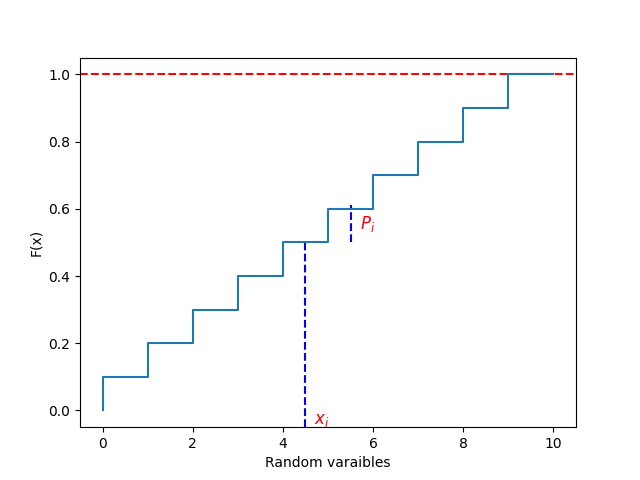
\includegraphics[width=\textwidth,height=5.5cm,keepaspectratio]{Figure_1}
		\caption{Staircase function}
		\label{fig1}
	\end{figure}
\end{frame}

% % Blocks frame
\section{Codes}
\begin{frame}{CODES}
    \begin{block}{Python}
         Download python code from - \href{https://github.com/jarpula-Bhanu/Assignment-8/blob/main/code/Graph.py}{Python}
    \end{block}

 \begin{block}{Beamer}
         Download Beamer code from - \href{https://github.com/jarpula-Bhanu/Assignment-8/blob/main/Assignment_8.tex.tex}{Beamer}
    \end{block}
\end{frame} 

\end{document}